%%%
% Plantilla de Presentación
% Modificación de una plantilla de Latex de LaTeXTemplates para adaptarla 
% al castellano y a las necesidades de escribir informática y matemáticas.
%
% Editada por: Mario Román
%
% License:
% CC BY-NC-SA 3.0 (http://creativecommons.org/licenses/by-nc-sa/3.0/)
%%%

%%%%%%%%%%%%%%%%%%%%%%%%%%%%%%%%%%%%%%%%%
% Beamer Presentation
% LaTeX Template
% Version 1.0 (10/11/12)
%
% This template has been downloaded from:
% http://www.LaTeXTemplates.com
%
% License:
% CC BY-NC-SA 3.0 (http://creativecommons.org/licenses/by-nc-sa/3.0/)
%
%%%%%%%%%%%%%%%%%%%%%%%%%%%%%%%%%%%%%%%%%

%----------------------------------------------------------------------------------------
%   PAQUETES Y CONFIGURACIÓN DEL DOCUMENTO
%----------------------------------------------------------------------------------------

\documentclass{beamer}

%% Configuración de la presentación
\mode<presentation> {
  %%% Selección de estilo
  % The Beamer class comes with a number of default slide themes
  % which change the colors and layouts of slides. Below this is a list
  % of all the themes, uncomment each in turn to see what they look like.

  % \usetheme{default}
  % \usetheme{AnnArbor}
  \usetheme{Antibes}
  %\usetheme{Bergen}
  %\usetheme{Berkeley}
  %\usetheme{Berlin}
  %\usetheme{Boadilla}
  %\usetheme{CambridgeUS}
  %\usetheme{Copenhagen}
  %\usetheme{Darmstadt}
  %\usetheme{Dresden}
  %\usetheme{Frankfurt}
  %\usetheme{Goettingen}
  %\usetheme{Hannover}
  %\usetheme{Ilmenau}
  %\usetheme{JuanLesPins}
  %\usetheme{Luebeck}
  % \usetheme{Madrid}
  %\usetheme{Malmoe}
  %\usetheme{Marburg}
  %\usetheme{Montpellier}
  %\usetheme{PaloAlto}
  %\usetheme{Pittsburgh}
  %\usetheme{Rochester}
  %\usetheme{Singapore}
  %\usetheme{Szeged}
  %\usetheme{Warsaw}

  %% Selección de color
  % As well as themes, the Beamer class has a number of color themes
  % for any slide theme. Uncomment each of these in turn to see how it
  % changes the colors of your current slide theme.

  % \usecolortheme{albatross}
  % \usecolortheme{beaver}
  %\usecolortheme{beetle}
  %\usecolortheme{crane}
  \usecolortheme{dolphin}
  %\usecolortheme{dove}
  %\usecolortheme{fly}
  %\usecolortheme{lily}
  %\usecolortheme{orchid}
  %\usecolortheme{rose}
  %\usecolortheme{seagull}
  %\usecolortheme{seahorse}
  %\usecolortheme{whale}
  %\usecolortheme{wolverine}

  %% Configuración del pie de línea
  %\setbeamertemplate{footline} % To remove the footer line in all slides uncomment this line
  %\setbeamertemplate{footline}[page number] % To replace the footer line in all slides with a simple slide count uncomment this line
  %\setbeamertemplate{navigation symbols}{} % To remove the navigation symbols from the bottom of all slides uncomment this line
}

%% Fuentes de tamaño arbitrario
\usepackage{lmodern}

%% Gráficos
\usepackage{graphicx} % Allows including images
\usepackage{booktabs} % Allows the use of \toprule, \midrule and \bottomrule in tables

%%% Castellano.
% noquoting: Permite uso de comillas no españolas.
% lcroman: Permite la enumeración con numerales romanos en minúscula.
% fontenc: Usa la fuente completa para que pueda copiarse correctamente del pdf.
% \usepackage[spanish,es-noquoting,es-lcroman]{babel}
\usepackage[utf8]{inputenc}
\usepackage[T1]{fontenc}
% \selectlanguage{spanish}

%Configuración de tablas
\usepackage{longtable}
\usepackage{rotating}
\usepackage{array}
\usepackage{multicol}
\usepackage{multirow}
\usepackage{booktabs}
\usepackage{float}

%----------------------------------------------------------------------------------------
%   TÍTULO
%----------------------------------------------------------------------------------------

\title[Método de Euler para sist. de ecuaciones]{Método de Euler para sistemas de ecuciones diferenciales} % The short title appears at the bottom of every slide, the full title is only on the title page

\author{María del Mar Ruiz Martín\\
        Antonio R. Moya Martín-Castaño\\
        Francisco Luque Sánchez} % Your name
\institute[UGR] % Your institution as it will appear on the bottom of every slide, may be shorthand to save space
{
  Universidad de Granada \\ % Your institution for the title page
}
\date{\today} % Date, can be changed to a custom date



\begin{document}

%% Diapositiva de título.
\begin{frame}
\titlepage 
\end{frame}

%% Diapositiva de contenidos.
% Throughout your presentation, if you choose to use \section{} and \subsection{} commands, 
% these will automatically be printed on this slide as an overview of your presentation

\section{Introducción}
\begin{frame}
  \frametitle{Introducción}
   % Table of contents slide, comment this block out to remove it
  Explicaremos el método de Euler para sistemas de ecuaciones diferenciales de primer orden. Por consiguiente, también servirá para resolver ecuaciones de orden superior. Este método no dejará de ser una extensión del método de Euler para ecuaciones diferenciales. \\
  
  Cabe nombrar que en la práctica no será muy utilizado, pues no aporta soluciones lo suficientemente buenas, es interesante su conocimiento por su gran simplicidad.
  
\end{frame}


\subsection{Partes del trabajo}
\begin{frame}
	\frametitle{Partes del trabajo:}
	\begin{itemize}
		\item Descripción general de un sistema de ecuaciones diferenciales
		\item Ecuaciones diferenciales de orden superior y reescritura como sistemas.
		\item Método de Euler para sistemas de ecuaciones diferenciales
		\item Estudio del error y análisis de la convergencia del método.
		
	\end{itemize}
\end{frame}

\section{Descripción general de un sistema de ecuaciones diferenciales}
\subsection{Concepto de ecuación diferencial}
\begin{frame}
	\frametitle{Concepto de ecuación diferencial:}
	
	Es una igualdad en la que interviene una variable independiente (\texttt{t}), una variable dependiente (x(\texttt{t})) y las sucesivas derivadas de la variable dependiente respecto de la independiente. de forma general, escribimos: 
	
	$$
	F(t,x,x', ..., x^{n)})=0
	$$
	
	También, nombrar que se definía \textit{orden} de la ecuación diferencial, como el mayor orden de derivación de la variable independiente que aparece en dicha ecuación.\\
	
	La \textit{solución} vendrá dada por un conjunto de ecuaciones que cumplan dichas condiciones.
\end{frame}

\subsection{PVI}
\begin{frame}
	\frametitle{Problema de valores iniciales}
	Se define un problema de valores iniciales (PVI), asociado a una ecuación diferencial a dicha ecuación, y el conjunto de $n$ valores (fijado $t_0$):
	
	$$
	x(t_0)=y_0, x'(t_0)=y_1, ...,  x^{n-1)}(t_0)=y_{n-1}
	$$
	
	Se dice que está \textit{bien planteado} si existe solución, es única y depende continuamente de los datos del problema.
	
\end{frame}

\subsection{Sistema de ecuaciones diferenciales}
\begin{frame}
	\frametitle{Sistema de ecuaciones diferenciales}
	
	Es un conjunto de ecuaciones diferenciales en las que aparecen una variable independiente, un conjunto de variables dependientes de dicha variable independiente y las sucesivas derivadas de dichas variables dependientes respecto de la independiente. 
	
	$$
	\begin{cases}
	F_1(t, x_1, x_1', ..., x_1^{n_1)}, ..., x_m, x_m', ..., x_m^{n_m)}) = 0 \\
	F_2(t, x_1, x_1', ..., x_1^{n_1)}, ..., x_m, x_m', ..., x_m^{n_m)}) = 0 \\
	\vdots \\
	F_r(t, x_1, x_1', ..., x_1^{n_1)}, ..., x_m, x_m', ..., x_m^{n_m)}) = 0
	\end{cases}
	$$
	
	Y de manera análoga a como hemos dicho anteriormente, podemos definir un PVI para este sistema.
\end{frame}

\begin{frame}
	\frametitle{Sistemas de primer orden}
	Dado que trabajaremos con sistemas de primer orden, a partir de ahora notaremos los sistemas del siguiente modo:
	
	$$
	\begin{cases}
	F_1(t, x_1, ..., x_m) = \frac{d x_1}{d t} \\
	F_2(t, x_1, ..., x_m) = \frac{d x_2}{d t} \\
	\vdots \\
	F_m(t, x_1, ..., x_m) = \frac{d x_m}{d t}
	\end{cases} 
	$$
	
	Y para el PVI asociado a dicho sistema: 
	
	$$ x_1(t_0) = y_1, x_2(t_0) = y_2, ..., x_m(t_0) = y_m $$
\end{frame}

\section{Ecuaciones diferenciales de orden superior y reescritura como sistemas}
\subsection{Reescritura}
\begin{frame}
	\frametitle{Reescritura de ecuaciones de orden superior}
Anteriormente hemos definido que es una ecuación diferencial de orden $n$. Ahora, veremos como reescribir una ecuación diferencial de orden n (con n>1), como un sistema:

Sea la ecuación diferencial de orden $n$: $ F(t, x, x', ..., x^{n)}) = 0 $. Podemos establecer los siguientes cambios de variable:

$$y_0 = x, y_1 = x', y_2 = x'', \dots, y_{n-1} = x^{n-1)}$$

Y con estas, la solución de $y_0$ en el sistema que queremos escribir, será la solución de nuestra ecuación diferencial.

\end{frame}

\begin{frame}
	
	Así, el sistema en el que hemos transformado la ecuación de orden $n$ sería el siguiente:
	
	$$
	\begin{cases}
	y_0' = x' = y_1\\
	y_1' = x'' = y_2\\
	\vdots\\
	y_{n-2}' = x^{n-1)} = y_{n-1}\\
	y_{n-1}' = x^{n)} = F(t, y_1, y_2, \dots, y_{n-1})
	\end{cases}
	$$
	
\end{frame}

\section{Método de Euler para sistemas de ecuaciones diferenciales}
\subsection{Recordatorio previo}
\begin{frame}
	\frametitle{Método de Euler para ecuaciones diferenciales}
	
	Antes de comentar el método de Euler para sistemas, recordemos en qué consistía el método de Euler para ecuaciones diferenciales. Dado un PVI bien planteado:
	
	$$
	\begin{cases}
	y'(t)=f(t,y(t)) \\ 
	y(t_0)=y_0, 
	\end{cases}
	$$
	
	si tomamos puntos en un intervalo [a,b], y tomamos un N natural, de forma que $h=(b-a)/n$
	Para cada $i=0,...,N$, tomamos los puntos:
	$t_i=a+ih$. Aplicando Taylor (centrado en $t_i$):
	
	
	
\end{frame}

\begin{frame}
	\frametitle{Método de Euler para ecuaciones diferenciales}
	$$
	y(t_{i+1})=y(t_i) + y'(t_i)(t_{i+1}-t_i) + y''(\xi_i)(t_{i+1}-t_i)^2/2
	$$ para algún $\xi_i$ entre $(t_i, ti_{i+1})$.\\
	Equivalentemente:
	
	$$
	y(t_{i+1})=y(t_i) + f(t_i,y(t_i))h + y''(\xi_i)h^2/2,
	$$
	
	Es decir: 
	
	$$
	y(t_{i+1})=y(t_i) + f(t_i,y(t_i))h + O(h^2).
	$$ 
	
\end{frame}

\begin{frame}
	\frametitle{Método de Euler para ecuaciones diferenciales}
	
	De este modo, el método aproxima cada $y_i$:
	
	$$
	\begin{cases}
	w_0=y_0\\
	w_{i+1}=w_i + hf(t_i,w_i)
	\end{cases}
	$$
\end{frame}

\subsection{Método de Euler para sistemas de ecuaciones diferenciales}
\begin{frame}
	\frametitle{Método de Euler para sistemas de ecuaciones diferenciales}
	
	Dicho esto, podemos observar, mediante una deducción análoga, cuál es el punto de partida del método de Euler para sistemas. Dado el sistema:
	
	$$
	\begin{cases}
	x_1'=F_1(t,x_1(t),...,x_n(t)) \\
	\vdots\\
	x_n'=F_n(t,x_1(t),...,x_n(t))
	\end{cases}
	$$
	
 para cada $j=1,...,n$, podemos hacer una aproximación de $w_{i,j} \approx x_j(t_i)$ de forma que:
 $$
 \begin{cases}
 w_{0,j}=x_{j,0} \\
 w_{i+1,j}=w_{i,j}+ hF_j(t_i,w_{i,j})
 \end{cases}
 $$ 
\end{frame}

\begin{frame}
	\frametitle{Método de Euler para sistemas de ecuaciones diferenciales}
	
	Y así, dado el siguiente sistema: $$
	X'(t)=F(t,X(t))
	$$
	donde X(t) es de la forma:
	
	\begin{equation*}
	X(t)=\begin{bmatrix}
	x_1(t) \\
	\vdots \\
	x_n(t)
	\end{bmatrix}
	\end{equation*}
	y F(t,X(t)):
	\begin{equation*}
	F(t,X(t))=\begin{bmatrix}
	F_1(t,x_1(t),...,x_n(t)) \\
	\vdots \\
	F_n(t,x_n(t),...,x_n(t))
	\end{bmatrix}
	\end{equation*}
	
	
	 
\end{frame}

\begin{frame}
	\frametitle{Método de Euler para sistemas de ecuaciones diferenciales}
	
	podemos expresar una aproximación $W_i \approx X(t_i)$ de a siguiente manera:
	$$
	\begin{cases}
	W_0=X(t_0)\\
	W_{i+1}=W_i + hF(t_i,W_i)
	\end{cases}
	$$
	donde $W_i$ es de la forma:
	
	\begin{equation*}
	W_i=\begin{bmatrix}
	w_1(t_i) \\
	\vdots \\
	w_n(t_i)
	\end{bmatrix}
	\end{equation*}
	
	
\end{frame}

\section{Estudio del error y análisis de la convergencia del método}
\subsection{Error local}
\begin{frame}
	\frametitle{Error local}
	\begin{block}{Teorema}
	El error local para el método de Euler es $O(h^2)$, donde $h$ es el tamaño del paso que hemos elegido para aplicar el método.
	\end{block}
	
	Para la demostración, supongamos que tenemos un valor exacto para un determinado $t_i$, entonces el error local para la siguiente iteración es $|| E_{i+1} || = ||X(t_{i+1}) - [X(t_{i}) + h*F(t_i, X_i)] ||$
	
	Si tomamos cada componente por separado y, además, realizamos el desarrollo de Taylor de $x_j(t_{i+1})$ con $j=1,...,n$, llegaríamos a que para cada $x_j$, el error cometido en un paso del método es:
	$$ e_{i+1, j} = | x_j(t_{i+1}) - \omega_{i+1, j} | = \frac{h^2}{2}*x''_j(\xi_{i+1, j}),\, \xi_{i+1, j} \in [t_i, t_{i+1}] $$	
	
\end{frame}

\begin{frame}
	\frametitle{Error local}
	
	Tenemos entonces que el vector de los errores lo podemos expresar como sigue:
	
	\begin{equation*}
	E_{i+1}=\begin{bmatrix}
	e_{i+1, 1} \\
	\vdots \\
	e_{i+1, n}
	\end{bmatrix}=\begin{bmatrix}
	\frac{h^2}{2}*x''_1(\xi_{i+1, 1}) \\
	\vdots \\
	\frac{h^2}{2}*x''_n(\xi_{i+1, n})
	\end{bmatrix}
	\end{equation*}
	
	Tomando ahora la norma euclídea del vector de los errores, tenemos que el error es $O(h^2)$
\end{frame}

\subsection{Error global}
\begin{frame}
	\frametitle{Error global}
	
	\begin{block}{Lema 1}
		Para toda $x \geq -1$ y para cualquier $m$ positiva, tenemos que $0 \leq (1 + x)^m \leq e^{mx}$
	\end{block}
	
	
	\begin{block}{Lema 2}
		Si $s$ y $t$ son números reales positivos, $\{a_i\}^k_{i=0}$ es una sucesión que satisface $ a_0 \geq -t/s$ y
		$$a_{i+1} \leq (1+s)a_i + t, \, \forall i=0, 1, ..., k$$
		entonces se tiene que
		$$a_{i+1} \leq e^{(i+1)s}\left( a_0 + \frac{t}{s}\right) - \frac{t}{s}$$
	\end{block}
	%Aplicando el teorema de Taylor:
	
	%$$ 0 \leq 1 + x \leq 1 + x + \frac{1}{2}x^2e^\xi = e^x $$
	
	%donde $0 < \xi < x$.
	
	%y como $1 + x \geq 0$:
	%$$ 0 \leq (1 + x)^m \leq (e^x)^m = e^{mx} $$
\end{frame}

\begin{frame}
	\frametitle{Error global}
	\begin{block}{Teorema}
		El error global del método de Euler para sistemas de ecuaciones es $O(h)$, donde $h$ es el tamaño de paso que hemos elegido al aplicar el método. 
	\end{block}
	
	El esquema general de esta demostración sería el siguiente. Suponiendo que cada función, $f_j(t, x_1, ..., x_n)$ es Lipschitziana en la variable $x_j$, con constante de Lipschitz $L_j$, y que para cada $x_j$ existe una constante $M_j$ tal que $| x''_j(t) | \leq M_j, \forall t \in [a,b]$.\\
	
	
\end{frame}

\begin{frame}
	\frametitle{Error global}

	Teniendo en cuenta el desarrollo de Taylor para $x_j(t_{i+1})$ y la aproximación $w_{i+1,j}$:
	
	$$
	x_j(t_{i+1}) - \omega_{i+1,j} = x_j(t_i) - \omega_{i,j} + h*[f_j(t_i, x_i, ..., x_n) $$
	$$- f_j(t_i, \omega_{i,1}, ..., \omega_{i,n})] + \frac{h^2}{2}*x''_j(\xi_j) $$
	Se cumple entonces que:
	$$ | x_j(t_{i+1}) - \omega_{i+1,j} | \leq | x_j(t_i) - \omega_{i,j} | + h|[f_j(t_i, x_i, ..., x_n) $$
	$$- f_j(t_i, \omega_{i,1}, ..., \omega_{i,n})]| + \frac{h^2}{2}*|x''_j(\xi_j)| $$
	
	
	
\end{frame}

\begin{frame}
	\frametitle{Error global}
	Y de aquí, teniendo en cuenta que $f_j$ es Lipschitziana:
	
	$$ | x_j(t_{i+1}) - \omega_{i+1,j} | \leq (1+hL_j)*| x_j(t_i) - \omega_{i,j} | + \frac{h^2*M_j}{2} $$
	
	Y aplicando el lema anterior y operando:
	
	$$ | x_j(t_{i+1}) - \omega_{i+1, j} | \leq \frac{hM_j}{2L_j}(e^{(t_{i+1}-a)L_j} - 1) $$
	Y dado que tomamos $j$ arbitrario, tenemos este resultado para todas las funciones $f_j$. Finalmente, tomando la norma euclídea de todos los errores globales, podemos concluir que el método es de orden $O(h)$.
\end{frame}

\begin{frame}
	\frametitle{Método de Euler para ecuaciones de orden superior}

\section{Ejercicios}


\begin{block}{Ejercicio 2}
	Dado el siguiente PVI, determinar el valor de x($\pi/4$)
	$$
	x''' = 2x'' - 2x'     % x(t) = e^tcos(t)
	$$
	$$
	x(0)=1, x'(0)=1, x''(0)=0
	$$
\end{block}

$$
\begin{cases}
y_0' = x' = y_1\\
y_1' = x'' = y_2\\
y_2' = x''' = 2y_2 - 2y_1
\end{cases}
$$

\end{frame}

\begin{frame}
	\frametitle{Método de Euler para ecuaciones de orden superior}

	\begin{figure}[H]
	\centering
	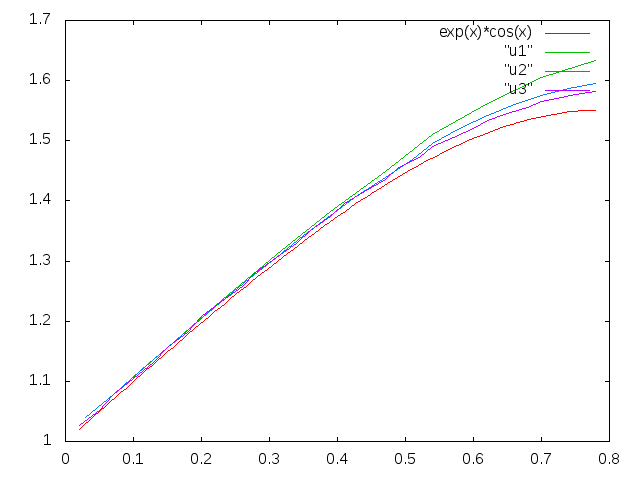
\includegraphics[scale=0.45]{img/graphic.png}
	\label{figura1}
	\caption{Aproximación para 25 (u1), 50 (u2) y 100 (u3) nodos} 
	\end{figure}


\end{frame}


\begin{frame}
	\frametitle{Método de Euler para ecuaciones de orden superior}

    \begin{table}[H]
        \centering
        \setlength\extrarowheight{3pt}
        
        \begin{tabular}{|c|c|c|c|c}
            \hline
            \textbf{h} & {\textbf{u($\pi$/4)}} & \textbf{Error} \\ 
            \hline
                $\pi$/120 & 1.581351427438043 & 0.030468230520017\\
            \hline
                $\pi$/240 & 1.566883575533628 & 0.016000378615602\\
            \hline
                $\pi$/360 & 1.561353411976403 & 0.010470215058378\\
            \hline
                $\pi$/480 & 1.558765635465628 & 0.007882438547603\\
            \hline
                $\pi$/600 & 1.557203467884946 & 0.0063202709669205\\
            \hline
                $\pi$/720 &  1.556204299202344 & 0.0053211022843184\\
            \hline
                $\pi$/840 & 1.555409383683734 & 0.0045261867657087\\
            \hline
        \end{tabular}
        
        \caption{Errores obtenidos con el método de Euler}           
    \end{table}

\end{frame}

\begin{frame}
\Huge{\centerline{Fin.}}
\end{frame}

%----------------------------------------------------------------------------------------

\end{document} 